% Plantilla realizada por Santiago Morante Cendrero

%parametros de tipo libro
\documentclass[10pt,a4paper,openany, ]{book}

%idioma espa�ol y acentos

\usepackage[english]{babel}
\usepackage[latin1]{inputenc}
\usepackage{setspace}
\spacing{1.5}

%algunos s�mbolos matem�ticos y paquete para usar subim�genes
\usepackage{amsmath}
\usepackage{amsfonts}
\usepackage{amssymb}
\usepackage{graphicx}
\usepackage{subfigure}
\usepackage{listings}
\usepackage{appendix}

%para generar �ndice con hiperv�nculos
\usepackage{hyperref}

%parametros del documento (sus propiedades)
\hypersetup{
    pdftitle={Arturo Arranz Mateo - TFG - a�o},
    pdfsubject={TFG - a�o},
    pdfauthor={Nombre del alumno},
    pdfkeywords={palabraclave1} {palabraclave2} {palabraclave3},
    colorlinks,
    citecolor=black,
    filecolor=black,
    linkcolor=black,
    urlcolor=black,
}

%empieza el documento
\begin{document}  

%elementos antes del trabajo en s� se meten dentro de frontmatter
\frontmatter

%cada incluye referencia a un archivo de tipo .tex
\begin{titlepage}
\begin{center}

%forma de introducir im�genes. el \\[0.5 cm] de final de l�nea introduce un salto de ese tama�o.
%width=1\textwidth indica el tama�o de la im�gen (valores entre 0-1). 
 
\includegraphics[width=1\textwidth]{figuras/cabecera.png}  \\[0.5 cm]

\large \textsc{Departamento de Ingenier�a Inform�tica} \\ [1 cm]

\large TRABAJO FIN DE GRADO\\[1 cm]

\huge \textsc{Reconocimento de acciones mediante kinect y aprendizaje autom�tico}\\[7 cm]

%flushleft alinea a la izquierda el texto
\begin{flushleft} \Large
\emph{Autor:} Arturo Arranz Mateo\\[0.5 cm]
\emph{Director:} nombre del director \\
\emph{Tutor:} nombre del tutor
\end{flushleft}

%rellena de blanco el resto de la p�gina para escribir abajo del todo
\vfill

% Bottom of the page
{\large Ciudad, Mes a�o}

\end{center}
\end{titlepage}

\begin{flushleft}

Copyright \copyright  a�o. Nombre del alumno

%ejemplo de licencia, se puede elegir cualquier otra

Esta obra est� licenciada bajo la licencia Creative Commons Atribuci�n-NoComercial-SinDerivadas 3.0 Unported (CC BY-NC-ND 3.0). Para ver una copia de esta licencia, visite http://creativecommons.org/licenses/by-nc-nd/3.0/deed.es o env�e una carta a Creative Commons, 444 Castro Street, Suite 900, Mountain View, California, 94041, EE.UU.

Todas las opiniones aqu� expresadas son del autor, y no reflejan necesariamente las opiniones
de la Universidad Carlos III de Madrid.

\end{flushleft}

\cleardoublepage

\begin{flushleft} \large
\textbf{T�tulo:} t�tulo del trabajo \\
\textbf{Autor:} nombre del alumno\\
\textbf{Director:} nombre del director \\ 
\textbf{Tutor:} nombre del tutor\\ [1 cm]

\end{flushleft} 

\begin{center} \LARGE
EL TRIBUNAL \\ [1 cm]
\end{center}

\begin{flushleft} \LARGE
Presidente: \\ [1 cm]
Vocal: \\ [1 cm]
Secretario: \\ [1.5 cm]
\end{flushleft}

\large
Realizado el acto de defensa y lectura del Trabajo Fin de Grado el d�a ....... de ....................   de ... en .........., en la Escuela Polit�cnica Superior de la Universidad Carlos III de Madrid, acuerda otorgarle la CALIFICACI�N de: \\ [2 cm]

\begin{center}
 \large VOCAL \\ [2.2 cm]
\end{center}

\begin{minipage}{0.5\textwidth}
 \begin{flushleft}
 \large SECRETARIO
\end{flushleft}
\end{minipage}
\begin{minipage}{0.5\textwidth}
\begin{flushright}
 \large PRESIDENTE
\end{flushright} 
\end{minipage}

\chapter{Agradecimientos}

Agradezco a ............

%chapter introduce un nuevo cap�tulo
\chapter{Resumen}

Este proyecto de resume en.................

\paragraph{Palabras clave:} palabraclave1, palabraclave2, palabraclave3.

\chapter{Abstract}

In this project...

\paragraph{Keywords:} keyword1, keyword2, keyword3.

%genera �ndice
\tableofcontents

%�ndice de figuras. Tambi�n se podr�a hacer uno de tablas (listoftables)
\listoffigures
 
%empieza la parte descriptiva del trabajo
\mainmatter
 
\chapter{Introducci�n}

En este cap�tulo...

%section es un apartado dentro de un chapter. Tambi�n existe subsection y subsubsection
\section{Estado del arte}

%las referencias a art�culos se ponen con \cite, 
%las referencias a im�genes \ref, 
%y las referencias a ecuaciones \eqref

Este tema.... Esto es un ejemplo de cita de un art�culo \cite{gonzalezeducational}.

%itemize es una lista. Cada t�rmino lleva delante un \item
\begin{itemize}
\item \textbf{ejemplo de lista de puntos}. Ejemplo.
\item \textbf{ejemplo2 de lista}. Ejemplo2.
\end{itemize} 

Ejemplo de referencia a figura (figura \ref{uc3m}).

%caption es el pie de foto, y label es el nombre que se da a la imagen para referenciarla despu�s. label no puede llevar acentos y no se muestra de cara al documento final (es s�lo interno).
\begin{figure}[h]
\centering

\includegraphics[width=0.45\textwidth]{figuras/uc3m}   
\caption{Logotipo de la UC3M \copyright UC3M}
\label{uc3m}
\end{figure}


\section{Motivaci�n del proyecto}

La idea...

\section{Estructura del documento}

A continuaci�n y para facilitar la lectura del documento, se detalla el contenido de cada cap�tulo.

\begin{itemize}
\item En el cap�tulo 1 se realiza una introducci�n.
\item En el cap�tulo 2 se hace un repaso...
\end{itemize}


\chapter{State of art}
\\
ARtajsdasdnasdfjaskodfcas
sdgfasdf

sfgad
fhsf
hgs
ghs
fghs
gs
afg
dfg
sdfg
dfg

\chapter{Analysis, design and implementation}


\section{Definition of the problem}

The problem to solve is \textbf{recognizing gestures in a 3-dimensional space}.
Those gestures will be the following:

\begin{itemize}
\item Slide left 
\item Slide right
\item Zoom in 
\item Zoom out
\item Point in order to select something
\end{itemize}

This problem arise several technical problems. Firstly about the data extraction: It is necessary to extract 3D dimensional analogous data and digitalize, recognize and track humans, abstract bodies into relevant points to track (wrist, head, elbow). 

Secondly there is several problems about the data analysis. Every gesture inside the same category is very hard to model, since is not always executed in the same way, not even from the same person. A simple example is the gesture of waiving, some people wave with the left hand, others with the right hand. Some wave very fast while other slower, or even not move from side to side. So we need a heuristic solution, a system able to generalize.

\section{My solution}

My solution will be the combination of the hardware Kinect and the Miscrosft Windows SDK for data extraction and machine learning techniques using the open-source Sklearn libraries. 


My approach will be a classification machine learning solution. Through training my system with enough amount of gesture samples, it will adjust to the given data to generalize and make clusters of each class. 

\section{Data extraction}

The solution selected for this purpose have been the hardware Kinect combined with the middleware, SDK, from Micrsoft Windows. The 3D image is constructed from the combination of a RGB camera with the depth sensor, which is a IR Emitter and a IR Depth sensor. Kinect is able to capture 30 frames per second. 
With the libraries from the SDK the body is tracked and abstracted as a skeleton, conformed by 20 joints. Each joint have x,y,z coordinates.

MEEETER IMAGEN DE KINECT kinect + joint?

SDK provides a basic interface, \textit{Skeleton Basics}, for tracking of bodies and visualization. I have changed it in order to record the gestures and store the  joint positions. Not all of them are relevant since the predefined gestures use only the arms. The stored joints are both hands, both elbows for recognizing gestures and spine neck for normalizing the bodies size.

With the new changed Skeleton Basics I am able to record each gesture manually and labelling in one of the mentioned categories. The output of this phase is a csv file with around 80 frames, where each frame is stored 6 pints and 1 label.

IMAGEN DE LA INTERFAZ 

\section{Preprocess Data}

\subsection{Attributes extraction}
Now that the relevant information about the skeleton have been extracted and stored it is necessary to clean and adapt for the machine learning algorithms. For the moment:

Gesture =( N_{frames} \times 6_{joint} \times 3_{coordinates} ) + 1 label

The first step is normalize respect the spine and make the system indifferent from the size of the person. Once normalize is done, the spine and neck joint are not necessary anymore. By this we reducing N_{frames} x 2 points, around 160 float points.

Gesture =( N_{frames} \times 4_{joint} \times 3_{coordinates} ) + 1 label

The attribute choice have been differential distances. Each succession of points have been chunked in n parts. Then is calculated the difference between the beginning of each part and the end. The differences are calculated in each axis 
Now the gesture is defined as:

Gesture = [n_{chuncks} \times 4_{joint} \times (\bigtriangleup x, \bigtriangleup y \bigtriangleup z)] + 1 label

The higher n the more accurate described will be the gesture. The lower n, the less amount of data the machine learning algorithms will have to handle. But the most important advantage of this step is that \textbf{the gestures are independent from the time}. Nevermind ,if it is executed faster or slower since it is chunked in the same parts. This assume that the movements are linear. Even thought that the real movements are not, it is a good approximation. 

\subsection{Standardization, or mean removal and variance scaling} 

Standardization of datasets is a common requirement for many machine learning estimators implemented in the sklearn libraries: they might behave badly if the individual feature do not more or less look like standard normally distributed data: Gaussian with zero mean and unit variance. 
For instance, if a feature has a variance that is orders of magnitude larger that others, it might dominate the learning function and make the estimator unable to learn from other features correctly as expected. 

This is achieved by removing the mean of each feature and scaling by dividing non-constant features by their standard deviation.

\section{Data Modelling}

The data is clean and prepared to be processed. Several machine learning algorithms have been tested. All of them are supervised techniques which mean that the data should be splitted into training data and testing data. 80 percent of the samples are going to be used for training each system and 20 percent to test the accuracy. An important step is mingling the samples so the testing and training datasets have samples from every category.\break

There is several classifications of the machine learning techniques. One of them is between parametric and not parametric models. 

A parametric algorithm has a fixed number of parameters.  A parametric algorithm is computationally faster, but makes stronger assumptions about the data; the algorithm may work well if the assumptions turn out to be correct, but it may perform badly if the assumptions are wrong.  A common example of a parametric algorithm is linear regression.
In contrast, a non-parametric algorithm uses a flexible number of parameters, and the number of parameters often grows as it learns from more data.  A non-parametric algorithm is computationally slower, but makes fewer assumptions about the data.

\subsection{Parametric algorithms}

\subsection*{Gaussian Naive Bayes}

The naive Bayes classifiers are based on the Bayes Theorem with a “naive” assumption that every pair of feature is independent with each other. Given a class variable y and a dependent vector x with n features the Bayes Theorem states:\break

FORMULA

This algorithm also assume that the features distribution is gaussian.

\subsection*{Linear Discriminant Analysis}


LDA is a non-parametric linear technique for classification. This method works by modelling the class conditional distribution P(f1,....fn| C) into a normal distribution, as the GNB does. Also each class Gaussian are assume to share the same covariance matrix. This lead to a linear decision boundary when comparing log-probability rations log(P(C=u| X)/P(C=k|X).

These classifier are an attractive choice since have a closed-form solution which can be easily computed.

GRAFICA COMPARANDO AMBOS

The results obtained for the parametric classifiers are:

\begin{itemize}
\item GNB training data: 84\% Testing data: 79\% 
\item LDA training data: 97\% Testing data: 93\%
\end{itemize}

The better results of LDA indicate that its assumptions fits better with the dataset. The feature independence that GNB assume appear not to be very accurate. However the datasets turns to work well with a gaussian distribution assumption, since both algorithm assume it. 

\subsection{Non Parametric algorithms}

The following classifiers do not make that strong assumptions of the dataset. Instead, they adapt to it, by tuning internal parameters, called hyperparameters. 

\subsection*{K Nearest Neighbours}

K-nn is a lazy non-parametric algorithms. In contrast to eager, lazy algorithms do not make generalization with training data, in other words there is not explicit training phase or it is very minimal. While other algorithms make generalizations and ride off of part of the training data, K-nn algorithm use all the training data to make predictions. However the the testing phase is very costly in term of time and memory. 

The KNN classifier labels an input sample \vv{Y} according to the following procedure: firstly it finds the K nearest vectors to \vv{Y} among the training data. This is usually performed with euclidean distances. Secondly it label \vv{Y} as the majority votes class of these nearest neighbours. 

\subsection*{Support Vector Machines}

Support Vector Machines is a binary classifier that aim to find the hyperplane over the feature space that maximize the margin, which is the distance from closer points to the hyperplane. This lead to a optimization(maximize margin) problem given some constraints(i.e. classify correctly), which is solved by Lagrange multipliers. 

There is several hyperparameters available for tuning the classifiers and avoiding overfitting. One of them is \textit{C}, which trade off misclassification for smoother decision boundary, by allowing outliers not being classify. Multiplying a point by \textit{C}, could be moved in the feature space in order to make it linearly separable. If C is too small any value could be moved and the decision boundary will not adjust to the real dataset. If \textit{C} is too big, the classifier would be too regularized and will not find a optimal solution. 

Another very powerful resource of SVMs is the \textit{kernel transformations}. If the input space is not linearly separable, it can be transformed in a higher dimension space through the kernel function. Two common used are the polynomic expansion and the radial basis function(rbf). Both add hyperparamters to the system, \textit{degree} for the polynomic kernel and \textit{gamma} for rbf.

\subsection*{Decision Tree}

\subsection*{Searching for estimator parameters}

As mentioned, the hyperparameters from the listed classifiers affect the learning performance. Therefore, it is necessary to tune them to find a optimal system. 
Evaluate them with the test set is a mistake since there is risk of overfitting, since the testing data would "leak" into the model. 
A simple approach for solving this problem, is dividing the training data into real training set and \textbf{validation set}, leaving test data for the final evaluation.  This validation set would be use to measure the accuracy of each hyperparameter combination tested.

However, this approach have two main issues. In one hand, we are consuming to much training data, which could be used to improve the model. On the other hand, the validation would rely on a particular random portion of the training set. 

A solution for this problem is a procedure called \textbf{cross-validation}. The test set is still separated for the final evaluation, but the validation set is no longer needed. Instead, the testing data is subdivided into K parts. Then each model is trained with K-1 parts and validate with the last. Each model is trained with all the combinations of K-1 part. The performance value is given by the average. 

There is several approaches for dividing the data in K parts. The one used in this project is the \textit{Stratified k-fold}, where each partition contains approximately the same percentage of samples of each targeted class as the complete set. Also, the K value used for every validation is 5. 

Finally is necessary to set which hyperparameters values will be used. A grid of parameters is set and then all the combinations are tested. The following hyperparameters have been tested:

For K-nn: K = [0,1,2,3,4,5,6,7,8,9,10,11]
For SVM: Kernel = ['linear', 'poly', 'rbf'], C = [0.001, 0.0046, 0.021, 0.1, 0.46, 2.15, 10, 46.4, 215, 1000]
Gamma rbf SVM:  0.000625  0.00125   0.0025    0.005     0.01      0.02   
Degree for poly SVM: 2 3 4

\begin{figure}
\centering
\begin{subfigure}
  \centering
  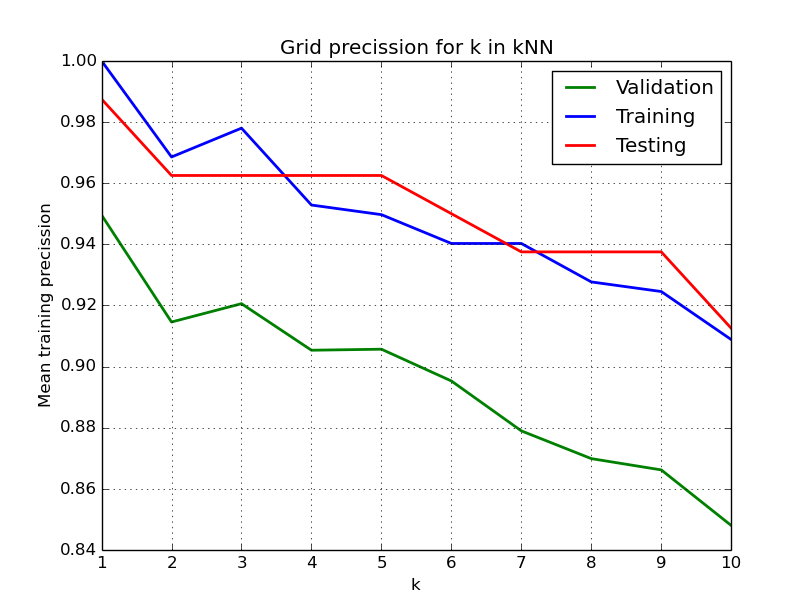
\includegraphics[width=1\textwidth]{figuras/cv_knn.png}
  \caption{A subfigure}
  \label{fig:sub1}
\end{subfigure}%
\begin{subfigure}
  \centering
  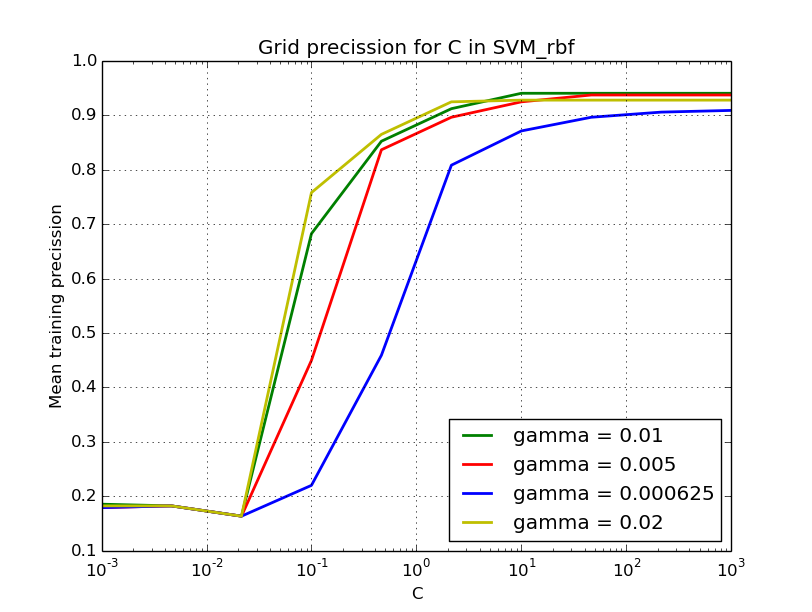
\includegraphics[width=1\textwidth]{figuras/cv_svmr.png}
  \caption{A subfigure}
  \label{fig:sub2}
\end{subfigure}
\caption{A figure with two subfigures}
\label{fig:test}
\end{figure}

The optimal parameters:
K = 1 for Knn
Linear SVM: C = 0.46
Ploy SVM: C = 10, degree = 2
Rbf SVM: C = 10, gamma = 0.01

\section{Evaluation}

\chapter{Conclusiones}

Se presentan a continuaci�n las conclusiones...

\section{Conclusi�n}

Una vez finalizado el proyecto...

\section{Desarrollos futuros}

Un posible desarrollo...

  
  %partes finales del trabajo: conclusiones, bibliografia y anexos
\backmatter


%estilo de bibliograf�a: plana, alfa...
\bibliographystyle{plain}

%genera doble hoja en blanco
%\cleardoublepage

%apartado de bibliograf�a
\addcontentsline{toc}{chapter}{Bibliograf�a}

%se incluye la bibliograf�a. Archivo de tipo .bib (bibtex)
\bibliography{bibliografia}

%fin del documento
\end{document}